\chapter{Analysis of Social Navigation in Modern Web Sites}
\label{chapter:analysis}

This chapter will include a survey and analysis of the data we've collected
which can be found in it's whole in
\appendixref{content.inventory}.

\section{Flickr}

\sidefigure{Flickr Photo Meta-data}{%
  Photo Meta-data,
  retrieved October 28, 2007, from
  \url{http://flickr.com/photos/benbengraves/187609810/}.
  \label{figure:scrsh.flickr.photo.detail.metadata}
}{%
  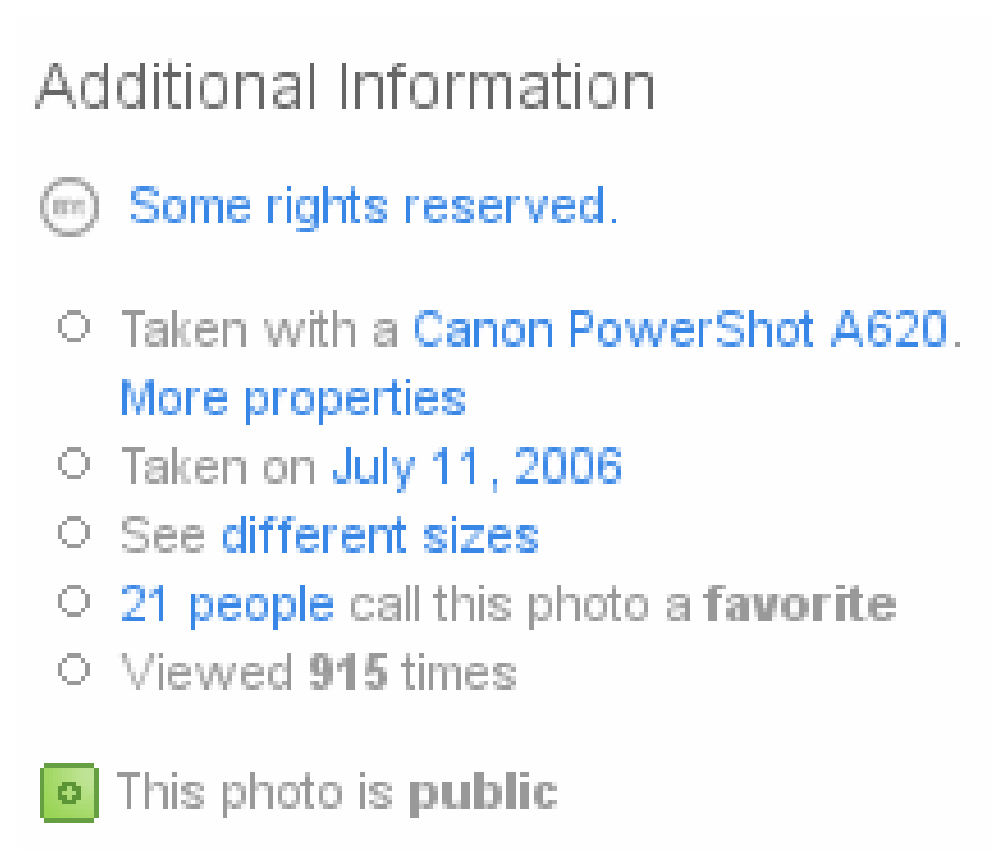
\includegraphics[width=0.9\marginparwidth]{scrsh_flickr_photo_metadata}
}

Flickr is a photo sharing site which are known to be on the cutting edge when
it comes to enabling new and innovating features in it's domain. Flickr has a
quite peculiar history as it started out as a massively multi player online
game. An environment for photo sharing within the game was added in 2004 which
quickly became more popular than the game itself. The focus of the company was
shifted and their new photo sharing community was bought by Yahoo! Inc. in
March 2005 \citep[p.~257]{livingston07}.

This subsequent
analysis of Flickr will be carried out as a registered user. One has to be
registered for interacting with the site in such a way that one leaves
persistent traces. The site has a open nature enabling anonymous access
to the majority of content.

\subsection{Thumbnails}

Already on the welcome page (\figureref{scrsh.flickr.welcome})
we're finding navigation links that are social of
nature. Four thumbnails functions as sample of the most recently uploaded
photos by other members of the community. One can either navigate straight to
a detailed page for each particular photo by clicking on the respective
thumbnail (Id 6, p.~\pageref{table:flickr.content.inventory.6})
or the profile of the uploader by clicking on their user
name (Id 7, p.~\pageref{table:flickr.content.inventory.7}). Such thumbnails
with minimal meta data (the uploader) are prevalent all over Flickr. Of the
120 pages we collected in our content inventory 26 of them contained
thumbnails. Most of these thumbnails
are giving users incentives to navigate using social means%
\sidenote[-4\onelineskip]{
  Apart from the few pages that only show a
  stream of your own thumbnails--when you're browsing your
  own photos by various methods.
}.
Which photos these thumbnails portray is dynamic. That is to say that other
users' actions--uploading a photo, tagging a photo, taking a photo with a
specific camera, collecting photos into sets, and adding photos to a certain
group--all determine the navigational choices you as a user is
presented with.

\subsection{Meta-data}

We arrive on a photo detail page as in
\figureref{scrsh.flickr.photo.detail}
if we utilize one of these thumbnails for navigation. In addition to comments
on the photo we find meta-data as in 
\figureref{scrsh.flickr.photo.detail.metadata}
Meta-data include the date the photo was taken, the manufacturer and the model
of the camera that was used which are all so called Exif%
\sidenote{Exchangeable Image File: a specification for image file format used
in digital cameras.}
data. Flickr utilize this data by enabling navigation based both on the
dates a picture was taken and by camera make and model. Say you're trying to
find a picture from your home town on a particularly beautiful summer day. By
using date of picture taking based navigation coupled with tags or
geographical data (which both will be discussed shortly) you're probably
increasing you chances of finding what you want. Camera make information could
be useful when looking at the quality of pictures taken with certain cameras
before purchasing one yourself.

\begin{figure}[b]
  \captionstyle{\raggedright}
  \begin{whole}
    \begin{minipage}[t]{0.475\wholewidth}
      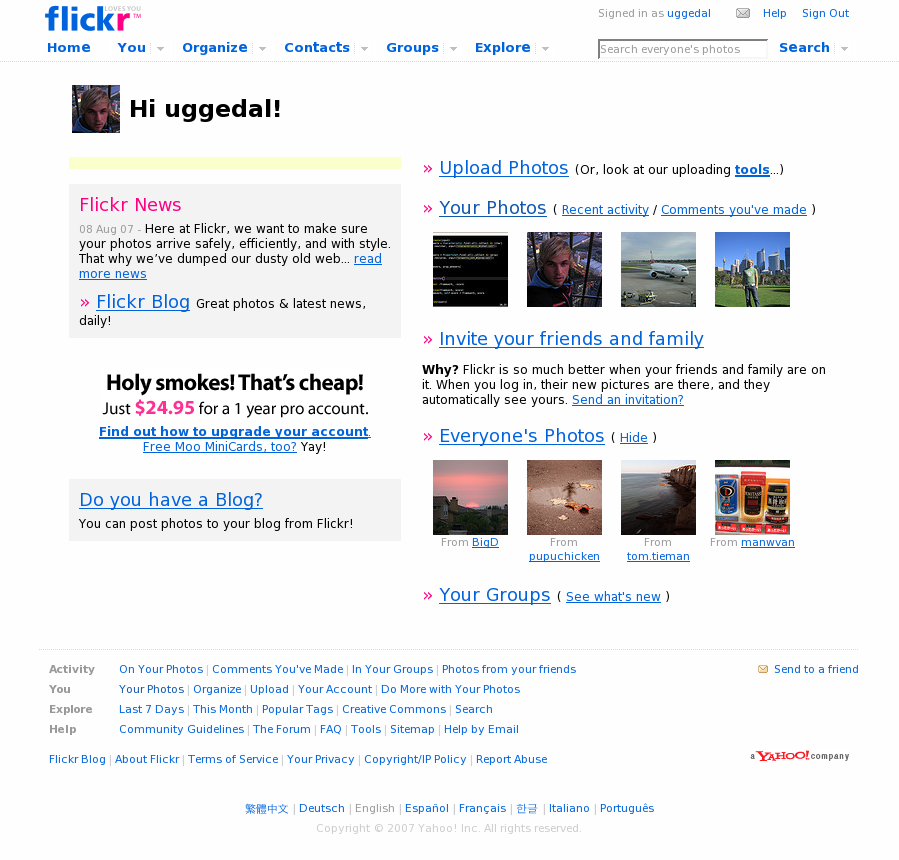
\includegraphics[width=\textwidth]{scrsh_flickr_welcome}
      \caption[Flickr Welcome Page]{%
         The Welcome Page,
         retrieved October 16, 2007, from \url{http://flickr.com}.}
      \label{figure:scrsh.flickr.welcome}
    \end{minipage}
    \hfill
    \begin{minipage}[t]{0.475\wholewidth}
      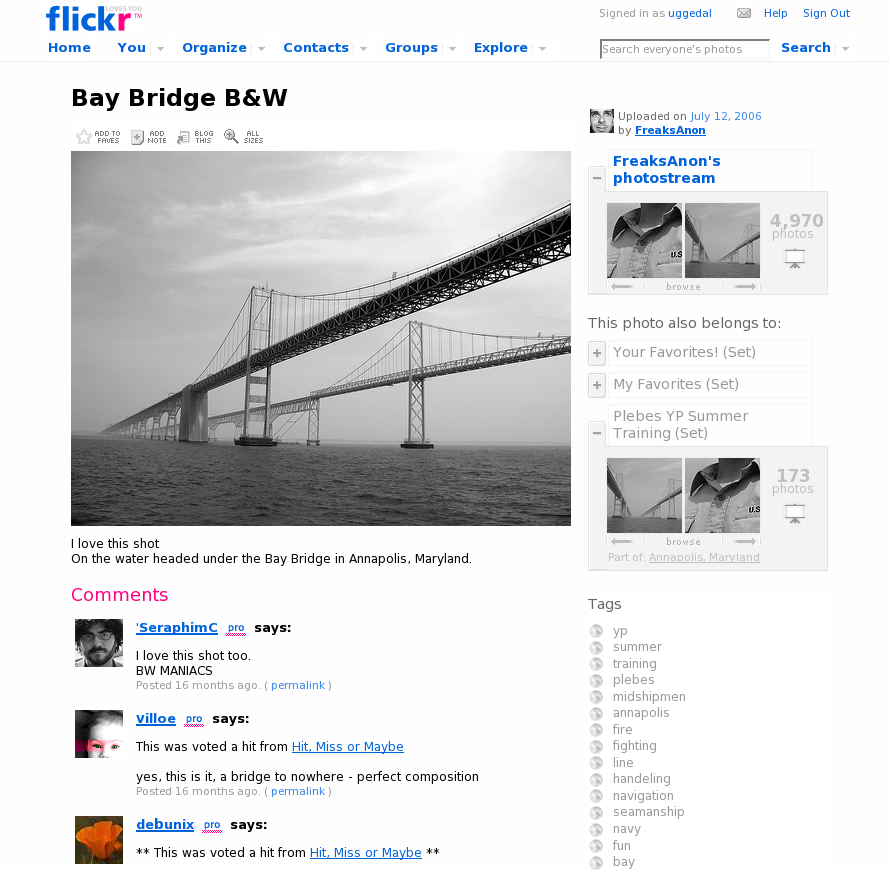
\includegraphics[width=\textwidth]{scrsh_flickr_photo_detail}
      \caption[Flickr Photo Detail Page]{%
         A Photo Detail Page,
         retrieved October 26, 2007, from
         \url{http://flickr.com/photos/benbengraves/187609810}.}
      \label{figure:scrsh.flickr.photo.detail}
    \end{minipage}
  \end{whole}
  \normalcaption
\end{figure}

\subsection{Folksonomy}
Of most importance
for Flickr, and indeed what makes Flickr a folksonomy, is it's tagging
abilities. Caterina Fake, co-founder of Flickr, explains it's importance:
``Tagging really revolutionized the way the product behaved.''
\citep[p.~261]{livingston07}
All
registered user can label anyone's photos by applying such short descriptive
tags. This collaborative process lay the ground work for other user's ability
to easily browse photos by topic.
\figureref{scrsh.flickr.tagcloud}
exemplifies how the user generated data trough tagging can be used as a
navigational aid. A so called \emph{tag cloud} is used to visualize the
popularity (and thereby importance) of the individual tags. The larger the
tag title, the more frequent the tag has been applied to photographs.

Tag clustering was released in the fall of 2005 \citep{butterfield05} as a way
to easier see the relationships between separate tags. For any given tag a
cluster of three related tags is generated and displayed to users when they
are browsing as seen in
\figureref{scrsh.flickr.photo.detail}.
Flickr algorithmically generates these listings based on what tags users tend
to use together for labeling a photo.

Tagging is a very flexible approach only hindered by users' imagination. In the
early days of Flickr there was no support for geographical data. Users soon
found a remedy for this by tagging photos with longitude and latitude. By
using the same technology we're using in our prototype application
(Greasemonkey) they were able to integrate Google Maps%
\sidenote{
  Available at \url{http://maps.google.com}
} in Flickr, enabling user's to place their photos on a map and automatically
generate geographical coordinate tags%
\sidenote{
  More info about the early days of \emph{geotagging} can be found on the
  remains of the Flickr Geotagging group, available at
  \url{flickr.com/groups/geotagging/}.
}.

\subsection{Geographical data}

In late August 2006 Flickr introduced geotagging abilities
\citep{butterfield06} by integrating mapping aspects from Yahoo! Maps%
\sidenote{
  Available at \url{http://maps.yahoo.com}.
}
Users could now place their photos on a
map to signify where they were captured.
% Finish description.
% Take screen shot.
% Write about the new places feature.
% Write and cite when proper geo data was incorporated.

\subsection{Interestingness}
% Cite collaborative filtering. Introduced in same blog post as clustering.

\begin{figure}[b]
  \begin{whole}
    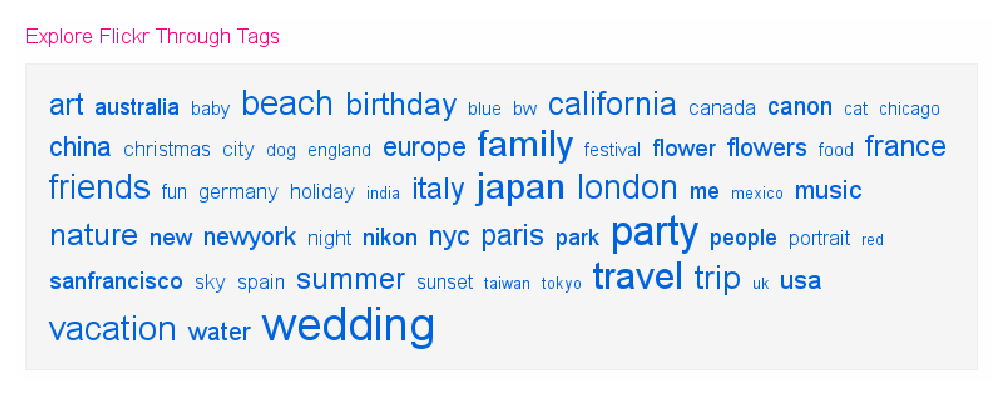
\includegraphics[width=\wholewidth]{scrsh_flickr_tagcloud}
    \caption[Flickr Tag Cloud]{%
       Tag Cloud,
       retrieved November 1, 2007, from \url{http://flickr.com/explore}.}
    \label{figure:scrsh.flickr.tagcloud}
  \end{whole}
\end{figure}

\begin{figure}[b]
  \begin{whole}
    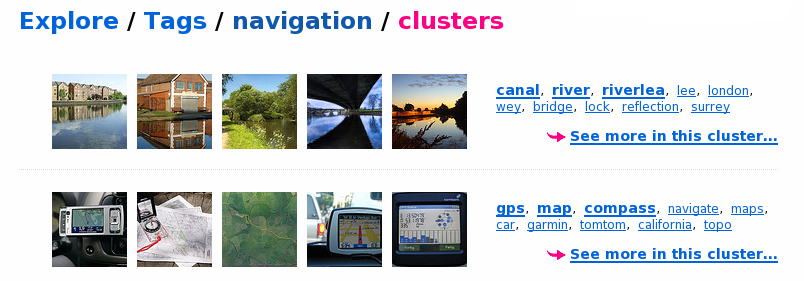
\includegraphics[width=\wholewidth]{scrsh_flickr_tagcluster}
    \caption[Flickr Tag Cluster]{%
       Tag Cluster,
       retrieved November 19, 2007, from
       \url{http://flickr.com/photos/tags/navigation/clusters/}.}
    \label{figure:scrsh.flickr.tagcluster}
  \end{whole}
\end{figure}

\section{Facebook}
\label{section:analysis.facebook}

\subsection{Profiles}

As we've seen pictures and their thumnails and titles are central in Flickr.
In the same way user names and thumnails of profile images are scattered all
trough facebook. This is no mystery as the dominant entity of Facebook is
persons and their profile much as pictures' essentialness for Flickr.

\section{Amazon}
